% Asal-usul (tidak pernah dicetak): lihat sources/outline_sources.md (Tahun 1: fluks larutan dan partikel; diagram Hjulström; kecepatan mengendap; laju denudasi). Nilai soal latihan dan soal dalam kalkulator skrap Buku 3 calc/ch20.py; data gambar dari figdata/bachelor-1/settling.py dan threshold.py. Erosi, transpor dan pengendapan adalah milik Buku 1 (kelas 5); muatan sedimen dalam tiga bentuk, laju denudasi dan pemantulan isostatik adalah milik Buku 2 (kelas 12), didirikan ulang di sini (muatan, laju denudasi) atau diingat kembali (pemantulan); debit dan daerah aliran sungai milik Buku 2 kelas 10; isostasi Airy milik bab 11; viskositas, hukum Stokes dan bilangan Reynolds milik buku-buku fisika (diakui, penunjuk). Kelas ukuran butir dan pemilahan termasuk dalam bab 21.
\chapter{Erosi dan transpor}\label{ch:b1:erosion-transport}

Setelah badai, sungai di bawah jembatan berwarna cokelat. Air yang kemarin jernih kini penuh lumpur, berputar di sekeliling pilar dan membawa ranting, dan di dasarnya, tak terlihat, kerikil saling membentur ketika bergulir. Setiap detik banjir membawa ton-ton tanah bersamanya. Di hilir, di belakang bendungan, lumpur yang sama mengendap di air tenang waduk, yang kehilangan sedikit volumenya setiap tahun; lebih jauh lagi, di muara sungai, ia menyebar ke laut sebagai gumpalan cokelat yang dapat terlihat dari angkasa. Bab ini memberi angka pada perjalanan itu: berapa banyak yang dibawa sungai dan dalam bentuk apa, seberapa cepat sebutir pasir tenggelam, arus seperti apa yang dibutuhkan untuk menggerakkannya, dan seberapa cepat, pada akhirnya, seluruh lanskap terkikis.

\begin{recall}
Erosi adalah pengikisan daratan dan pengangkutan pecahannya; pengendapan adalah peletakannya di tempat pembawanya melambat (Buku~1, kelas~5). Sebuah sungai membawa muatan sedimennya sebagai \omterm{def:b1:erosion-transport:load}{muatan dasar}, \omterm{def:b1:erosion-transport:load}{muatan melayang} dan \omterm{def:b1:erosion-transport:load}{muatan terlarut}; \omterm{def:b1:erosion-transport:denudation}{laju denudasi} suatu wilayah adalah ketebalan batuan yang diangkut darinya per satuan waktu, dalam meter per juta tahun; ketika erosi menghilangkan ketebalan $e$ dari \omterm{def:b1:layered-earth:layers}{kerak}, pemantulan isostatik membuat permukaan turun hanya sebesar $e(1 - \rho_c/\rho_m)$ (Buku~2, kelas~12). Debit sungai adalah volume air yang melewati suatu penampang per satuan waktu, dan daerah aliran sungainya adalah luas yang memasoknya (Buku~2, kelas~10). Dalam \omterm{prop:b1:isostasy-gravity:airy}{isostasi Airy} \omterm{def:b1:layered-earth:layers}{kerak} mengapung di atas \omterm{def:b1:layered-earth:layers}{mantel} dengan akar yang sebanding dengan reliefnya (\cref{prop:b1:isostasy-gravity:airy}). \omterm{def:b1:weathering-clays:hydrolysis}{Hidrolisis} silikat mengirim ion dan silika terlarut ke sungai (\cref{def:b1:weathering-clays:hydrolysis}). Viskositas dinamis $\mu$ suatu fluida mengukur resistensinya terhadap geseran, dan viskositas kinematik adalah $\nu = \mu/\rho$; sebuah bola berdiameter $d$ yang bergerak perlahan dengan kecepatan $w$ melalui fluida merasakan hambatan $3\pi\mu d w$ (hukum Stokes); bilangan Reynolds $w d/\nu$ membandingkan inersia dengan gaya viskos, dan aliran di sekeliling bola halus selama ia tetap kecil (buku-buku fisika).
\end{recall}

\section{Fluks larutan dan partikel}\label{sec:b1:erosion-transport:fluxes}

Sungai menghilangkan daratan dengan dua cara: sebagai materi dalam larutan, produk \omterm{def:b1:weathering-clays:weathering}{pelapukan kimia}, dan sebagai butiran padat, produk \omterm{def:b1:weathering-clays:weathering}{pelapukan fisik} serta residu tak larut dari \omterm{def:b1:weathering-clays:weathering}{pelapukan kimia}. Keduanya berpindah secara berbeda, dan butiran itu sendiri berpindah dengan dua cara.

\begin{definition}[Muatan terlarut, muatan melayang, muatan dasar]\label{def:b1:erosion-transport:load}
Muatan sungai adalah materi yang dibawanya melewati suatu penampang, dalam tiga bagian yang berbeda menurut cara mereka berpindah. \emph{Muatan terlarut}\index{muatan terlarut} adalah materi dalam larutan, yakni ion dan silika terlarut, yang bergerak bersama air dengan kecepatannya sendiri. \emph{Muatan melayang}\index{muatan melayang} terdiri dari butiran yang ditopang di dalam aliran oleh turbulensinya, sebagian besar lempung, lanau dan pasir halus, yang bergerak hampir dengan kecepatan air dan jarang menyentuh dasar. \emph{Muatan dasar}\index{muatan dasar} terdiri dari butiran yang bergulir, meluncur atau melompat di sepanjang dasar, sering bersentuhan dengannya, dan jauh lebih lambat daripada air.
\end{definition}

\begin{omfigure}
\begin{tikzpicture}[font=\footnotesize, >={Stealth[length=4pt]}]
% schematic: the three loads of a river (side view) and the forces on a bed grain
\fill[omDef!12] (0,0) rectangle (9,3.2);
\draw[omDef!80!black, thick] (0,3.2) -- (9,3.2);
\node[anchor=south west, omDef!80!black] at (0,3.2) {permukaan air};
% flow profile arrows (velocity grows upward)
\foreach \y/\l in {0.35/0.5, 0.8/0.9, 1.4/1.15, 2.1/1.3, 2.8/1.4} {\draw[->, black!55] (0.25,\y) -- ++(\l,0);}
\draw[black!55] (0.25,0.12) -- (0.25,3.05);
\node[anchor=north west, black!65, align=left] at (0.2,-0.15) {profil kecepatan\\ aliran};
% bed
\fill[black!12] (0,-0.05) rectangle (9,0.12);
\foreach \x in {0.1,0.45,...,8.9} {\fill[black!45] (\x,0.0) circle[radius=0.09];}
% dissolved load: ions
\foreach \x/\y/\s in {2.3/2.7/+, 3.1/1.9/-, 4.0/2.85/+, 4.7/2.2/-, 5.6/2.75/+, 6.3/1.85/+, 7.2/2.6/-, 8.2/2.2/+, 2.7/1.2/-, 7.8/1.3/-} {\node[circle, draw=omThm, inner sep=0.2pt, minimum size=7pt, font=\tiny, text=omThm] at (\x,\y) {$\s$};}
% suspended load: fine grains, denser near the bed
\foreach \x/\y in {2.1/1.5, 2.6/0.9, 3.0/2.5, 3.4/0.6, 3.7/1.4, 4.2/0.8, 4.4/1.9, 4.9/0.55, 5.2/1.2, 5.5/2.1, 5.9/0.7, 6.1/1.5, 6.6/0.9, 6.9/2.3, 7.4/0.6, 7.6/1.7, 8.0/0.85, 8.5/1.4, 3.9/0.45, 5.0/0.35, 6.4/0.4, 2.4/0.45, 8.6/0.5} {\fill[brown!75!black] (\x,\y) circle[radius=0.05];}
% bed load: rolling and hopping grains
\fill[black!60] (3.2,0.27) circle[radius=0.15];
\draw[->, black!70] (3.0,0.55) arc[start angle=150, end angle=30, radius=0.25];
\fill[black!60] (5.6,0.25) circle[radius=0.12];
\draw[->, black!70, densely dashed] (4.6,0.2) .. controls (4.9,0.9) and (5.3,0.7) .. (5.55,0.4);
\fill[black!60] (4.6,0.22) circle[radius=0.06];
% labels
\node[omThm, anchor=west] at (9.2,2.5) {muatan terlarut: ion};
\node[brown!75!black, anchor=west] at (9.2,1.5) {muatan melayang:};
\node[brown!75!black, anchor=west] at (9.2,1.1) {lempung, lanau, pasir halus};
\node[black!75, anchor=west] at (9.2,0.4) {muatan dasar: bergulir,};
\node[black!75, anchor=west] at (9.2,0.0) {meluncur, melompat};
\draw[->, thick, black!70] (6.8,3.55) -- node[above] {aliran} (8.6,3.55);
% inset: forces on a grain resting on two others; it pivots about its downstream contact
\begin{scope}[xshift=11.8cm, yshift=-2.2cm]
  \fill[black!12] (-1.2,-0.4) rectangle (1.2,0);
  \fill[black!40] (-0.6,-0.15) circle[radius=0.28]; \fill[black!40] (0.6,-0.15) circle[radius=0.28];
  \fill[black!65] (0,0.166) circle[radius=0.4];
  \draw[->, thick, omDef!80!black] (0,0.166) -- (0,1.15) node[above] {angkat};
  \draw[->, thick, omThm] (0,0.166) -- (1.05,0.166) node[right] {seret};
  \draw[->, thick, black] (0,0.166) -- (0,-0.8) node[below] {berat dalam air};
  \draw[->, thick, black!60] (-1.4,0.85) -- (-0.5,0.85) node[pos=0, left] {aliran};
  \fill[red!60!black] (0.353,-0.020) circle[radius=0.045];
  \node[font=\scriptsize, anchor=north west, black!70] at (0.5,-0.4) {poros};
\end{scope}
\end{tikzpicture}

{\small Tiga muatan sungai, dilihat dari samping (skematis, tidak dalam skala). Aliran paling cepat di dekat permukaan dan melambat hingga nol di dasar. Ion tersebar di seluruh kedalaman; butiran melayang dibawa oleh pusaran, lebih banyak di dekat dasar; butiran \omterm{def:b1:erosion-transport:load}{muatan dasar} bergulir, meluncur atau melompat pendek. Kanan: gaya-gaya pada sebutir di dasar. Seret dan angkat aliran cenderung menggulingkannya melewati tetangga hilirnya, di sekitar titik kontak; beratnya dalam air menahannya.}
\label{fig:b1:erosion-transport:loads}
\end{omfigure}

Batas antara kedua muatan padat tidak ditentukan oleh ukuran butir: ia bergantung pada aliran. Banjir yang membawa pasir dalam suspensi meninggalkannya di dasar, sebagai \omterm{def:b1:erosion-transport:load}{muatan dasar}, ketika ia surut; lempung terhalus, di sisi lain, tetap dalam suspensi di hampir arus apa pun dan hampir tidak pernah ditemukan di dasar sungai yang mengalir. Setiap muatan diukur sebagai fluks, yakni massa per satuan waktu melalui suatu penampang sungai.

\begin{proposition}[Fluks suatu muatan]\label{prop:b1:erosion-transport:flux}
Misalkan $c$ adalah konsentrasi suatu \omterm{def:b1:erosion-transport:load}{muatan terlarut} atau melayang (massa per satuan volume air) dan $u$ kecepatan air, keduanya bervariasi di seluruh penampang luas $A$. (1)~Fluks sesaat muatan melalui penampang adalah
\[
  F = \iint_A c\,u\,\mathrm dA = \overline{c}_Q\,Q,
\]
di mana $Q = \iint_A u\,\mathrm dA$ adalah debit dan $\overline{c}_Q$ konsentrasi rerata yang diberi bobot kecepatan. (2)~Selama periode $T$ ketika debit $Q(t)$ dan konsentrasi $C(t)$ sungai bervariasi, massa yang terbawa adalah
\[
  M = \int_0^T Q\,C\,\mathrm dt = T\left(\overline{Q}\;\overline{C} +
  \operatorname{cov}(Q, C)\right),
\]
di mana garis atas menunjukkan rerata terhadap waktu dan $\operatorname{cov}(Q, C)$ adalah rerata dari $(Q - \overline{Q})(C - \overline{C})$. Hasil kali debit rerata dan konsentrasi rerata hanya memberi massa yang benar jika keduanya tidak berkorelasi.
\end{proposition}

\begin{proof}
(1)~Dalam waktu $\mathrm dt$ air yang melintasi luas kecil $\mathrm dA$ dari penampang
mengisi volume $u\,\mathrm dA\,\mathrm dt$, yang membawa massa
$c\,u\,\mathrm dA\,\mathrm dt$; menjumlahkan di seluruh penampang memberi $F$, dan
$\overline{c}_Q$ didefinisikan sebagai $F/Q$. (2)~Tulis $Q = \overline{Q} + Q'$ dan $C =
\overline{C} + C'$, dengan fluktuasi $Q'$ dan $C'$ yang memiliki rerata nol selama
periode itu. Maka $QC = \overline{Q}\,\overline{C} + \overline{Q}\,C' + Q'\,\overline{C}
+ Q'C'$; kedua suku tengah rata-ratanya nol, dan rerata $Q'C'$ adalah
kovariansi.
\end{proof}

Kovariansi penting untuk \omterm{def:b1:erosion-transport:load}{muatan melayang}. Konsentrasinya naik tajam dalam banjir, ketika hujan membilas tanah ke sungai dan aliran yang lebih cepat mengangkat butiran dari dasar, sehingga $Q$ dan $C$ naik bersama-sama: sebagian besar sedimen tahunan sungai lewat dalam beberapa hari banjir, dan kampanye pengambilan sampel yang melewatkannya, atau konsentrasi rerata dikalikan debit rerata, akan meremehkan muatan. \omterm{def:b1:erosion-transport:load}{Muatan terlarut} berperilaku sebaliknya: banjir mengencerkannya, dan konsentrasinya tertinggi pada debit rendah, ketika sungai diisi oleh air tanah yang telah lama bersentuhan dengan batuan.

\begin{method}[Muatan tahunan sungai dari pengukuran debit]\label{met:b1:erosion-transport:gauging}
\begin{enumerate}
  \item Catat debit secara terus-menerus di stasiun pengukuran.
  \item Ambil sampel air pada banyak debit, termasuk banjir, dan ukur massa sedimen per liter (dengan penyaringan dan penimbangan) serta massa setiap spesi terlarut.
  \item Beri bobot konsentrasi dengan debit pada saat pengambilan sampel untuk mendapatkan konsentrasi rerata berbobot aliran, atau cocokkan konsentrasi sebagai fungsi debit dan terapkan pada seluruh rekaman.
  \item Kalikan dengan volume total air tahun itu, atau jumlahkan $Q\,C\,\Delta
        t$ sepanjang rekaman (\cref{prop:b1:erosion-transport:flux}).
  \item Tambahkan \omterm{def:b1:erosion-transport:load}{muatan dasar}, yang terlewatkan oleh pengambil sampel air, dari pengukuran terpisah atau sebagai fraksi perkiraan.
  \item Untuk \omterm{def:b1:erosion-transport:load}{muatan terlarut}, buang apa yang tidak berasal dari batuan: garam yang dibawa hujan dan, untuk bikarbonat, karbon yang diambil dari udara (\cref{ch:b1:weathering-clays}).
\end{enumerate}
\end{method}

\begin{omfigure}
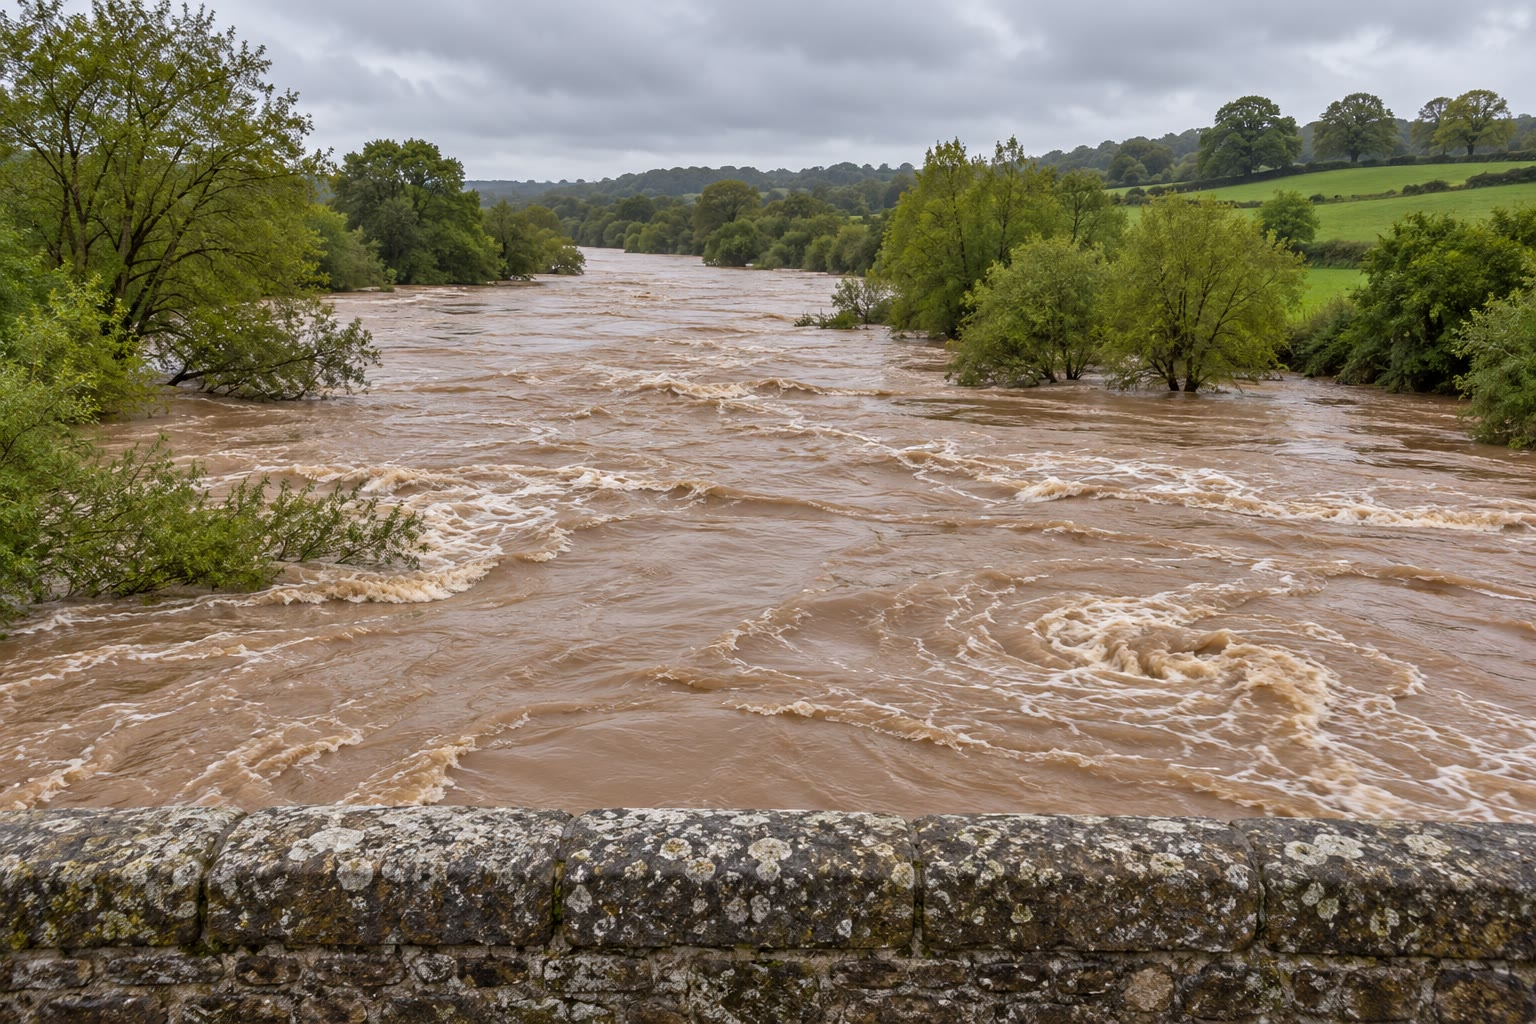
\includegraphics[height=5.1cm]{images/book3/ai/b1-muddy-river.jpg}\hfill
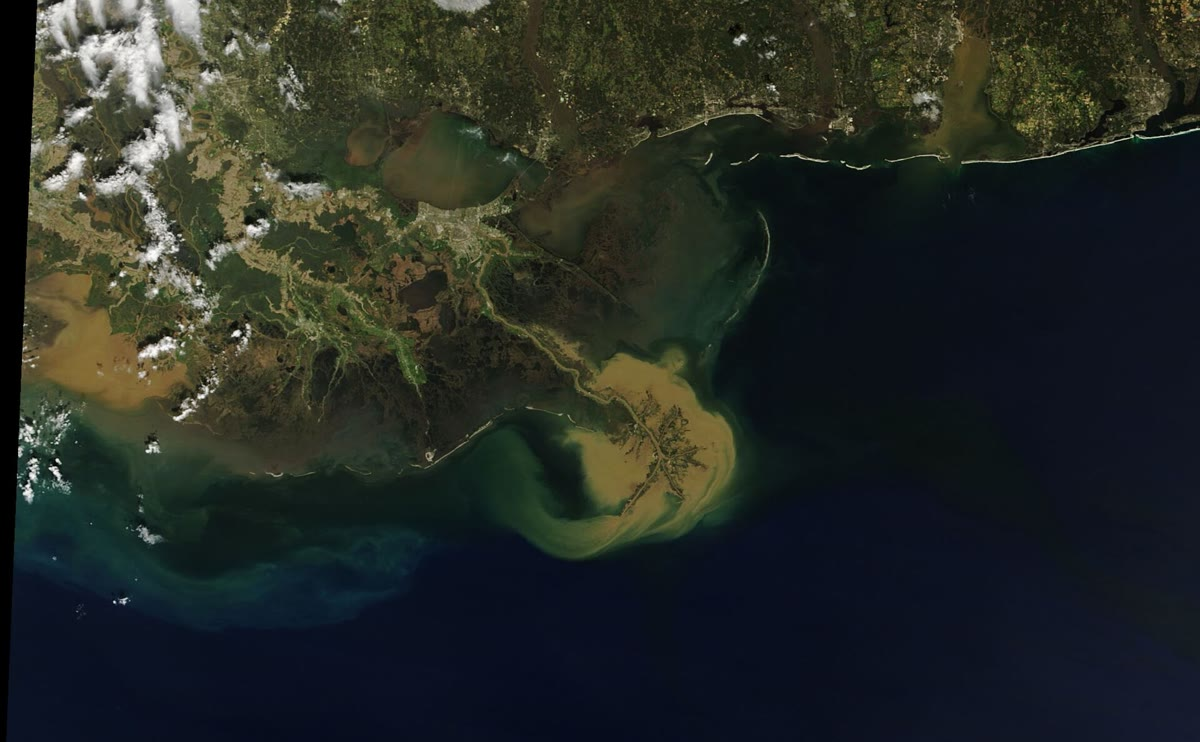
\includegraphics[height=5.1cm]{images/book3/b1-mississippi-plume.jpg}
{\small Kiri: sungai yang banjir membawa air cokelat yang sarat sedimen (ilustrasi AI). Kanan: gumpalan banjir Mississippi yang tumpah ke Teluk Meksiko di sekitar deltanya, terlihat oleh instrumen MODIS pada satelit Terra pada 4~Maret 2018; lumpur melayang mewarnai laut menjadi cokelat dan hijau, dan angin tenggara mendorong gumpalan itu ke barat laut. Citra NASA Earth Observatory oleh Joshua Stevens, domain publik, melalui Wikimedia Commons.}
\label{fig:b1:erosion-transport:plume}
\end{omfigure}
% ledger: commons:mississippi-plume

\emph{Sungai-sungai dunia.} Sebelum pengaruh manusia, sungai-sungai dunia diperkirakan membawa \qty{14}{Gt} sedimen melayang setahun ke laut pesisir, \qty{15.5}{Gt} bersama \omterm{def:b1:erosion-transport:load}{muatan dasar}. Manusia telah mengubah kedua ujung perjalanan itu: pertanian dan penggundulan hutan meningkatkan erosi tanah, menambahkan sekitar \qty{2.3}{Gt} setahun ke sungai, sementara waduk menahan sedimen: waduk besar memerangkap sekitar \qty{20}{\percent} dari fluks dan waduk kecil \qty{6}{\percent} lainnya, dan lebih dari \qty{100}{Gt} sedimen kini berada di belakang bendungan yang sebagian besar dibangun dalam lima puluh tahun terakhir. Efek bersihnya adalah penurunan: fluks modern sekitar \qty{12.6}{Gt} setahun.
% ledger: syvitski:flux

\begin{dated}{2005}
Angka fluks sedimen melayang, sebelum dan sesudah pengaruh manusia, berasal dari sebuah model global sedimen sungai yang diterbitkan pada 2005. Bendungan telah dibangun sejak itu.
\end{dated}
% ledger: syvitski:flux

\omterm{def:b1:erosion-transport:load}{Muatan terlarut} lebih kecil. Sebuah kompilasi klasik analisis sungai, dibuat pada 1963, menempatkan materi terlarut yang dikirim sungai-sungai dunia ke laut sekitar \qty{3.9}{Gt} setahun, sekitar \qty{30}{\percent} dari fluks melayang modern, pada konsentrasi rerata \qty{120}{mg} per liter. Bikarbonat membentuk hampir separuhnya, \qty{58}{mg.L^{-1}}, diikuti oleh kalsium, silika, sulfat, klorida dan natrium. Sebagian dari muatan itu tidak berasal dari batuan: banyak bikarbonat membawa karbon yang diambil dari udara atau tanah, dan sebagian klorida serta natrium berasal dari garam laut yang dibawa hujan. Sungai-sungai individual bervariasi luas di sekitar rerata ini.
% ledger: livingstone:world-dissolved, syvitski:flux

\emph{Anggaran sedimen suatu cekungan.} Tidak setiap butir yang tererosi di suatu daerah aliran sungai mencapai muaranya. Tanah yang tersapu dari sebuah ladang dapat berhenti di kaki lereng, pasir dapat tersimpan selama berabad-abad di dataran banjir dan gosong sungai, dan sebuah waduk dapat menahan sebagian besar yang memasukinya. Muatan yang diukur di muara adalah keseimbangan anggaran: apa yang tererosi di lereng dan dari tebing sungai, dikurangi apa yang tersimpan di sepanjang jalan, ditambah apa yang diambil kembali dari simpanan lama. Selama beberapa dekade pengukuran debit, keseimbangan ini dapat jauh dari laju erosi jangka panjang, ke arah mana pun, yang menjadi salah satu alasan bagi metode lain dalam \cref{sec:b1:erosion-transport:denudation}.

\section{Kecepatan mengendap}\label{sec:b1:erosion-transport:settling}

Sebutir butiran lebih padat daripada air dan tenggelam. Apakah sungai dapat membawanya, dan di mana ia akan diendapkan, bergantung pertama-tama pada seberapa cepat ia tenggelam.

\begin{definition}[Kecepatan mengendap]\label{def:b1:erosion-transport:settling}
\emph{Kecepatan mengendap}\index{kecepatan mengendap} $w_s$ suatu butiran adalah kecepatan tetap pada saat ia jatuh melalui air diam, ketika seret air menyeimbangkan berat terendamnya, yaitu beratnya dikurangi daya apung air yang dipindahkannya.
\end{definition}

Butiran yang dilepaskan di air diam dipercepat sampai seretnya, yang tumbuh seiring kecepatannya, menyeimbangkan berat terendamnya; untuk butiran pasir atau lanau ini memerlukan sebagian kecil dari sedetik, sehingga \omterm{def:b1:erosion-transport:settling}{kecepatan mengendap} adalah kecepatan saat ia jatuh hampir sepanjang jalan. Dengan massa jenis $\rho_s$ butiran dan $\rho$ air, tulislah $R = (\rho_s - \rho)/\rho$ untuk massa jenis terendam relatif.

\begin{proposition}[Pengendapan Stokes]\label{prop:b1:erosion-transport:stokes}
Sebuah bola berdiameter $d$ dan massa jenis $\rho_s$ yang jatuh perlahan melalui air dengan massa jenis $\rho$ dan viskositas dinamis $\mu$, menurut hukum Stokes, memiliki \omterm{def:b1:erosion-transport:settling}{kecepatan mengendap}
\[
  w_s = \frac{(\rho_s - \rho)\,g\,d^2}{18\,\mu} = \frac{R\,g\,d^2}{18\,\nu}.
\]
Hukum ini berlaku selama bilangan Reynolds butiran $w_s d/\nu$ berada di bawah sekitar 1, yakni untuk diameter di bawah $d_1 = \left(18\,\nu^2/(R\,g)\right)^{1/3}$.
\end{proposition}

\begin{proof}
Berat bola adalah $\rho_s g\,\pi d^3/6$ dan daya apungnya $\rho g\,\pi d^3/6$, sehingga berat terendamnya adalah $(\rho_s - \rho)\,g\,\pi d^3/6$.
Pada \omterm{def:b1:erosion-transport:settling}{kecepatan mengendap} ia sama dengan seret $3\pi\mu d\,w_s$:
\[
  (\rho_s - \rho)\,g\,\frac{\pi d^3}{6} = 3\pi\mu d\,w_s
  \quad\Longrightarrow\quad
  w_s = \frac{(\rho_s - \rho)\,g\,d^2}{18\,\mu},
\]
dan membagi pembilang dan penyebut dengan $\rho$ memberi bentuk kedua.
Bilangan Reynolds pada kecepatan ini adalah $R g d^3/(18\nu^2)$, yang sama dengan 1 untuk $d = d_1$ dan tumbuh sebagai $d^3$.
\end{proof}

Untuk kuarsa, dengan massa jenis \qty{2650}{kg.m^{-3}}, dalam air pada \qty{20}{\celsius},
dengan massa jenis \qty{998.2}{kg.m^{-3}} dan viskositas \qty{1.0016}{mPa.s}: $R =
1.65$, $\nu = \qty{1.003e-6}{m^2.s^{-1}}$, dan dengan $g =
\qty{9.81}{m.s^{-2}}$ batasnya adalah $d_1 = \qty{0.104}{mm}$, pasir halus. Di bawahnya, hukum Stokes memberi \omterm{def:b1:erosion-transport:settling}{kecepatan mengendap} lanau dan lempung: butiran lanau
berdiameter \qty{10}{\micro m} tenggelam dengan \qty{9.0e-5}{m.s^{-1}}, \qty{1}{m} dalam sekitar tiga jam;
sebuah partikel lempung berdiameter \qty{2}{\micro m} dengan
\qty{3.6e-6}{m.s^{-1}}, \qty{1}{m} dalam \num{3.2}~hari. Partikel lempung alami berupa
keping, bukan bola, dan tenggelam lebih lambat lagi. Air sedalam \qty{5}{m}, benar-benar diam, akan membutuhkan enam belas hari untuk bersih dari lempung semacam itu; sungai yang mengalir, yang pusarannya terus mengaduknya, tidak pernah bersih, dan itulah sebabnya lumpur terhalus mencapai laut.
% ledger: hom:quartz, nist:water, const:gn

Di atas $d_1$ seret tumbuh lebih cepat daripada sebanding dengan kecepatan: air yang mengalir melewati butiran memisah di belakangnya menjadi jejak, dan pada bilangan Reynolds besar seret sebanding dengan kuadrat kecepatan. Eksperimen pada butiran alami dirangkum dalam satu rumus tunggal yang menyatukan kedua rezim.

\begin{proposition}[Hukum pengendapan gabungan]\label{prop:b1:erosion-transport:combined}
\omterm{def:b1:erosion-transport:settling}{Kecepatan mengendap} butiran alami dengan diameter ayakan $d$ adalah, untuk semua
ukuran,
\[
  w_s = \frac{R\,g\,d^2}{C_1\,\nu + \sqrt{0.75\,C_2\,R\,g\,d^3}},
\]
dengan $C_1 = 18$ dan $C_2 = 1.0$.
\end{proposition}
\admitted
% ledger: fc:settling

Hukum ini berasal dari Ferguson dan Church, yang mencocokkannya dengan \omterm{def:b1:erosion-transport:settling}{kecepatan mengendap} terukur dari pasir alami. Untuk butiran kecil akar kuadratnya dapat diabaikan dan ia tereduksi menjadi hukum Stokes; untuk butiran besar suku pertama penyebutnya dapat diabaikan dan $w_s \to \sqrt{4 R g d/(3 C_2)}$, yang tumbuh hanya sebagai akar kuadrat ukuran. Konstanta bergantung pada bentuk butiran: $C_2 = 0.4$ menggambarkan bola halus, nilai yang lebih besar menggambarkan butiran yang lebih bersudut, yang menghadapi seret lebih besar. Kedua hukum berpisah jalan di atas \qty{0.1}{mm}. Untuk butiran \qty{1}{mm} hukum gabungan memberi \qty{0.126}{m.s^{-1}}, tujuh kali lebih kecil dari hukum Stokes; untuk kerikil berdiameter \qty{10}{mm}, \qty{0.46}{m.s^{-1}} melawan \qty{90}{m.s^{-1}} yang tak bermakna (diagram di bawah).
% ledger: fc:settling

\begin{omfigure}
\begin{tikzpicture}[font=\small]
% settling velocity of quartz grains in water at 20 C (figdata/bachelor-1/settling.py)
\begin{axis}[width=11cm, xmode=log, ymode=log, xmin=0.001, xmax=10, ymin=1e-8, ymax=10, height=8cm,
    xlabel={diameter butiran $d$ (\si{mm})}, ylabel={kecepatan mengendap (\si{m.s^{-1}})},
    ytick={1e-8,1e-6,1e-4,1e-2,1},
    legend style={at={(0.03,0.97)}, anchor=north west, font=\footnotesize}, legend cell align=left,
    grid=major, grid style={black!10}]
  \addplot[omDef, thick, dashed] table[x=d_mm, y=w_stokes] {figdata/out/bachelor-1-settling-curves.dat};
  \addplot[omThm, very thick] table[x=d_mm, y=w_fc] {figdata/out/bachelor-1-settling-curves.dat};
  \legend{hukum Stokes, hukum gabungan (butiran alami)}
  \draw[black!55, densely dotted] (axis cs:0.1037,1e-7) -- (axis cs:0.1037,10);
  \node[font=\scriptsize, anchor=west, align=left, black!75] at (axis cs:0.115,1e-6) {bilangan Reynolds butiran\\ $= 1$};
  \node[font=\scriptsize, black!70] at (axis cs:0.002,3e-8) {lempung};
  \node[font=\scriptsize, black!70] at (axis cs:0.016,3e-8) {lanau};
  \node[font=\scriptsize, black!70] at (axis cs:0.35,3e-8) {pasir};
  \node[font=\scriptsize, black!70] at (axis cs:4.5,3e-8) {kerikil};
  \draw[black!40] (axis cs:0.0039,1e-8) -- (axis cs:0.0039,1e-7);
  \draw[black!40] (axis cs:0.0625,1e-8) -- (axis cs:0.0625,1e-7);
  \draw[black!40] (axis cs:2,1e-8) -- (axis cs:2,1e-7);
\end{axis}
\end{tikzpicture}

{\small \omterm{def:b1:erosion-transport:settling}{Kecepatan mengendap} butiran kuarsa dalam air pada \qty{20}{\celsius} terhadap diameternya, keduanya pada skala logaritmik: hukum Stokes dan hukum gabungan untuk butiran alami, dihitung. Pada skala ini hukum Stokes berupa garis lurus dengan gradien 2. Keduanya sepakat untuk lanau dan lempung; di atas sekitar \qty{0.1}{mm}, ketika bilangan Reynolds butiran melampaui 1, seret jejak memperlambat butiran kasar. Tanda-tanda di bagian bawah menandai batas kelas ukuran butir, pada \qty{3.9}{\micro m} ($1/256$~mm), \qty{62.5}{\micro m} ($1/16$~mm) dan \qty{2}{mm}.}
\label{fig:b1:erosion-transport:settling}
\end{omfigure}
% ledger: fc:settling, usgs:wentworth-phi

Dalam rentang diagram, dari lempung terhalus hingga kerikil kasar, \omterm{def:b1:erosion-transport:settling}{kecepatan mengendap} membentang delapan orde besaran. Inilah alasan pertama mengapa sungai memilah sedimennya: arus yang melambat segera menjatuhkan kerikilnya, pasirnya dalam jarak meter, lanaunya dalam jarak kilometer, dan membawa lempungnya ke danau atau ke laut. Kelas ukuran butir dan pemilahan sedimen menjadi pokok bahasan bab berikutnya (\cref{ch:b1:clastic-sediments}).

\section{Ambang gerak dan diagram Hjulström}\label{sec:b1:erosion-transport:threshold}

Sebutir butiran yang diam di dasar sungai digerakkan oleh gaya air yang mengalir di atasnya. Gaya itu diukur dengan tegangan.

\begin{definition}[Tegangan geser dasar, kecepatan geser]\label{def:b1:erosion-transport:bed-shear}
\emph{Tegangan geser dasar}\index{tegangan geser dasar} $\tau_b$ suatu aliran adalah gaya per satuan luas yang dikerjakannya pada dasarnya, sejajar dengan dasar, searah aliran. Kecepatan geser adalah $u_* = \sqrt{\tau_b/\rho}$, sebuah kecepatan yang mengukur tegangan yang sama.
\end{definition}

\omterm{def:b1:erosion-transport:bed-shear}{Tegangan geser dasar} tidak dapat dibaca dari alat ukur arus, tetapi dalam aliran tunak ia mengikuti dari keseimbangan gaya.

\begin{proposition}[Hasil kali kedalaman dan gradien]\label{prop:b1:erosion-transport:depth-slope}
Dalam aliran tunak dan seragam dengan kedalaman $h$ di sepanjang saluran lebar dengan gradien kecil $S$, \omterm{def:b1:erosion-transport:bed-shear}{tegangan geser dasar} adalah
\[
  \tau_b = \rho\,g\,h\,S .
\]
\end{proposition}

\begin{proof}
Perhatikan air di atas sepotong dasar sepanjang $L$ searah aliran dan lebar satu satuan, saluran itu sangat lebar sehingga tebingnya dapat diabaikan. Aliran
tunak dan seragam, sehingga air ini tidak dipercepat dan gaya-gayanya seimbang. Gaya tekanan pada sisi hulu dan sisi hilirnya sama besar dan berlawanan arah, karena kedalamannya sama di kedua sisi. Di sepanjang aliran tersisa komponen berat,
$\rho g h L \sin\beta$, dengan $\beta$ sebagai sudut dasar, dan gesekan dasar, $\tau_b L$, yang melawannya. Maka $\tau_b
= \rho g h \sin\beta$, dan untuk sudut kecil $\sin\beta \approx \tan\beta = S$.
\end{proof}

Sebuah sungai sedalam \qty{2}{m} pada gradien \num{0.001}, satu meter jatuh per kilometer, memiliki $\tau_b = 998.2 \times 9.81 \times 2 \times 0.001 =
\qty{19.6}{Pa}$, dan kecepatan geser \qty{0.140}{m.s^{-1}}. Dalam saluran yang tidak lebar, tebing mengambil bagiannya dari gesekan, dan kedalaman digantikan oleh jari-jari hidrolik, yakni luas penampang dibagi keliling basahnya (\cref{exo:b1:erosion-transport:5}).

\emph{Gaya pada sebutir.} Aliran mendorong sebutir di dasar dengan seretnya dan mengangkatnya dengan aliran yang lebih cepat di atasnya (inset pada gambar pertama bab
ini). Kedua gaya bekerja pada luas butiran, sehingga keduanya berskala sebagai $\tau_b
d^2$; butiran melawan dengan berat terendamnya, yang berskala sebagai
$(\rho_s - \rho) g d^3$. Rasio keduanya adalah ukuran alami kekuatan aliran untuk butiran tertentu.

\begin{definition}[Parameter Shields, ambang gerak]\label{def:b1:erosion-transport:threshold}
\emph{Parameter Shields}\index{parameter Shields} suatu aliran dengan \omterm{def:b1:erosion-transport:bed-shear}{tegangan geser dasar} $\tau_b$ di atas butiran berdiameter $d$ dan massa jenis $\rho_s$ adalah
\[
  \theta = \frac{\tau_b}{(\rho_s - \rho)\,g\,d}.
\]
\emph{Ambang gerak}\index{ambang gerak} butiran adalah \omterm{def:b1:erosion-transport:bed-shear}{tegangan geser dasar}, atau nilai $\theta_c$ dari parameter Shields, pada saat mereka mulai bergerak.
\end{definition}
% ledger: hecras:thresholds

Nilai kritis $\theta_c$ diukur di saluran uji, dan pengukurannya jatuh pada satu kurva ketika diplot terhadap ukuran butir tak berdimensi yang menggabungkan butiran dan fluida.

\begin{proposition}[Kurva ambang Soulsby dan Whitehouse]\label{prop:b1:erosion-transport:soulsby}
Untuk butiran berdiameter $d$ pada dasar datar, dengan
$D_* = d\,\left(R\,g/\nu^2\right)^{1/3}$, \omterm{def:b1:erosion-transport:threshold}{parameter Shields} kritisnya adalah
\[
  \theta_c = \frac{0.3}{1 + 1.2\,D_*} + 0.055\left(1 - e^{-0.02\,D_*}\right),
\]
dan \omterm{def:b1:erosion-transport:bed-shear}{tegangan geser dasar} kritisnya adalah $\tau_c = \theta_c\,(\rho_s - \rho)\,g\,d$.
\end{proposition}
\admitted
% ledger: hecras:thresholds

Untuk butiran kasar $\theta_c$ cenderung ke \num{0.055}: kerikil bergerak ketika \omterm{def:b1:erosion-transport:bed-shear}{tegangan geser dasar} mencapai sekitar seperduapuluh berat terendam sebuah lapisan butiran setebal satu diameter, per satuan luas. Rumus transpor sedimen yang memakai ambang konstan mengambil nilai dari \num{0.03} hingga \num{0.047}, yang terakhir dalam rumus \omterm{def:b1:erosion-transport:load}{muatan dasar} klasik Meyer-Peter dan Müller. Untuk pasir halus $\theta_c$ naik lagi, hingga
\num{0.077} pada \qty{0.1}{mm}: butiran kecil berada dalam lapisan air yang lambat dan kental dekat dasar, dan terlindung oleh tetangganya. Minimumnya,
\num{0.030}, jatuh dekat \qty{0.7}{mm}. Dalam pascal ambang selalu tumbuh seiring ukuran (diagram di bawah): \qty{0.13}{Pa} untuk pasir \qty{0.1}{mm},
\qty{0.51}{Pa} pada \qty{1}{mm}, \qty{9.0}{Pa} pada \qty{10}{mm}, \qty{57}{Pa} untuk kerakal \qty{64}{mm}.
% ledger: hecras:thresholds

\begin{omfigure}
\begin{tikzpicture}[font=\small]
% threshold of motion of quartz grains in water at 20 C (figdata/bachelor-1/threshold.py, Soulsby and Whitehouse)
\begin{axis}[name=a, width=6.9cm, height=6cm, xmode=log, xmin=0.0625, xmax=100, ymin=0, ymax=0.12,
    xlabel={diameter butiran $d$ (\si{mm})}, ylabel={parameter Shields kritis $\theta_c$},
    yticklabel style={/pgf/number format/fixed, /pgf/number format/precision=2},
    grid=major, grid style={black!10}, title={\footnotesize (a) tak berdimensi}]
  \addplot[omThm, very thick] table[x=d_mm, y=theta] {figdata/out/bachelor-1-threshold-shields.dat};
  \draw[black!50, dashed] (axis cs:0.0625,0.055) -- (axis cs:100,0.055) node[pos=0.7, above, font=\scriptsize, black!70] {$0.055$};
\end{axis}
\begin{axis}[at={(a.east)}, anchor=west, xshift=2.0cm, width=6.9cm, height=6cm, xmode=log, ymode=log,
    xmin=0.0625, xmax=100, ymin=0.05, ymax=200,
    xlabel={diameter butiran $d$ (\si{mm})}, ylabel={tegangan geser dasar kritis $\tau_c$ (\si{Pa})},
    grid=major, grid style={black!10}, title={\footnotesize (b) dalam pascal}]
  \addplot[omDef, very thick] table[x=d_mm, y=tau_cr] {figdata/out/bachelor-1-threshold-shields.dat};
\end{axis}
\end{tikzpicture}

{\small \omterm{def:b1:erosion-transport:threshold}{Ambang gerak} butiran kuarsa dalam air pada \qty{20}{\celsius}, dari kurva Soulsby dan Whitehouse, dihitung dari batas pasir halus (\qty{0.0625}{mm}) hingga ukuran kerakal. (a)~\omterm{def:b1:erosion-transport:threshold}{Parameter Shields} kritis hampir konstan untuk kerikil dan naik untuk pasir halus. (b)~\omterm{def:b1:erosion-transport:bed-shear}{Tegangan geser dasar} kritis tumbuh hampir sebanding dengan diameter untuk kerikil.}
\label{fig:b1:erosion-transport:threshold}
\end{omfigure}
% ledger: hecras:thresholds

\begin{example}[Apa yang digerakkan sungai]\label{ex:b1:erosion-transport:river}
Di sungai sedalam \qty{2}{m} pada gradien \num{0.001}, $\tau_b =
\qty{19.6}{Pa}$. Untuk butiran \qty{20}{mm}, $\theta = 19.6/(1651.8 \times
9.81 \times 0.020) = 0.060$, sedikit di atas ambang mereka \num{0.055}: mereka
bergerak. Untuk butiran \qty{40}{mm}, $\theta = 0.030$, setengah dari ambang: mereka
tetap diam. Sungai menggerakkan dasarnya hingga kerikil kasar; untuk pasir \qty{1}{mm},
$\theta = 1.21$, hampir empat puluh kali lipat ambang \num{0.031}.
\end{example}

\emph{Masuk ke suspensi.} Begitu bergerak, sebutir melompat di sepanjang dasar atau terangkat ke dalam aliran, bergantung pada apakah pusaran, yang kecepatannya berorde kecepatan geser, dapat menopangnya melawan pengendapannya.

\begin{proposition}[Kriteria suspensi]\label{prop:b1:erosion-transport:suspension}
Sebutir dengan \omterm{def:b1:erosion-transport:settling}{kecepatan mengendap} $w_s$ dapat tetap dalam suspensi dalam aliran turbulen hanya jika beberapa pusaran naik lebih cepat daripada ia tenggelam. Karena kecepatan naik pusaran berorde kecepatan geser $u_*$, suspensi dimulai ketika $u_*$ mendekati $w_s$ dan berkembang penuh ketika $u_*$ melampauinya; bab ini mengambil $u_* = w_s$ sebagai batas suspensi.
\end{proposition}
\admitted
% ledger: bagnold:suspension

Dalam sungai pada contoh, $u_* = \qty{0.140}{m.s^{-1}}$, yang oleh hukum pengendapan gabungan memberi butiran \qty{1.16}{mm}: pasir yang lebih halus dari sekitar satu milimeter berpindah dalam suspensi, pasir yang lebih kasar dan kerikil sebagai \omterm{def:b1:erosion-transport:load}{muatan dasar}. Argumen ini kembali ke Bagnold, yang mencatat bahwa butiran \qty{0.1}{mm} atau lebih kecil tersuspensi penuh begitu mereka bergerak, sementara butiran yang lebih besar dari \qty{1}{mm} membutuhkan \omterm{def:b1:erosion-transport:bed-shear}{tegangan geser dasar} yang berkali-kali lipat dari ambangnya. Ketika banjir surut dan $u_*$ turun, pasir kasar jatuh kembali ke dasar lebih dulu.

\emph{Dari tegangan ke kecepatan rerata.} Yang mudah diukur, atau diperkirakan, di sungai adalah kecepatan rerata-nya. Dalam aliran turbulen di atas dasar yang dikasarkan oleh butiran berdiameter $d$, saluran lebar berkedalaman $h$ memiliki kecepatan rerata $U = u_*\left(6.25 + 5.75\log_{10}(h/d)\right)$, hukum yang ditetapkan oleh Keulegan pada 1938 dari eksperimen Nikuradse dan Bazin, sehingga \omterm{def:b1:erosion-transport:threshold}{ambang gerak} sesuai dengan kecepatan rerata kritis
\[
  U_c = \left(6.25 + 5.75\,\log_{10}\frac{h}{d}\right)\sqrt{\theta_c\,R\,g\,d},
\]
dan batas suspensi, $u_* = w_s$, ke $U_s = \left(6.25 +
5.75\log_{10}(h/d)\right) w_s$. Keduanya bergantung pada kedalaman, tetapi hanya melalui sebuah logaritma.
% ledger: keulegan:mean-velocity, bagnold:suspension

Kecepatan ambang karena itu termasuk pada satu kedalaman dan satu himpunan hukum: dihitung untuk kedalaman lain, atau dibaca dari pengukuran lain, hasilnya berbeda. Diplot terhadap ukuran butir, bentuknya kokoh tetapi nilainya tidak, dan \omterm{def:b1:erosion-transport:bed-shear}{tegangan geser dasar}, yang tidak bergantung pada kedalaman dengan cara yang sama, adalah ukuran yang lebih baik tentang apa yang dapat dilakukan suatu aliran. Kecepatan tetap lebih intuitif, dan cara klasik untuk menggambarkannya adalah diagram.

\begin{definition}[Diagram Hjulström]\label{def:b1:erosion-transport:hjulstrom}
Sebuah \emph{diagram Hjulström}\index{diagram Hjulström} memplot kecepatan rerata suatu aliran terhadap diameter butiran, pada skala logaritmik, dan membagi bidang menjadi medan-medan tempat butiran yang diam tererosi, butiran yang sudah bergerak tetap terangkut, dan butiran yang bergerak diendapkan.
\end{definition}
% ledger: hjulstrom:curve

\begin{omfigure}
\begin{tikzpicture}[font=\small]
% Hjulstrom-type diagram for a flow 1 m deep (figdata/bachelor-1/threshold.py); the hatched
% cohesive field is schematic (its lower edge, 30 cm/s, is not computed)
\begin{axis}[width=12cm, height=8.4cm, xmode=log, ymode=log, xmin=0.001, xmax=100, ymin=0.1, ymax=3000,
    xlabel={diameter butiran $d$ (\si{mm})}, ylabel={kecepatan aliran rerata (\si{cm.s^{-1}})},
    unbounded coords=jump, grid=major, grid style={black!10}]
  \addplot[draw=none, name path=dep] table[x=d_mm, y=u_dep] {figdata/out/bachelor-1-threshold-hjul.dat};
  \addplot[draw=none, name path=bot] coordinates {(0.001,0.1) (100,0.1)};
  \addplot[fill=omDef!14, draw=none] fill between[of=dep and bot];
  \fill[pattern=north east lines, pattern color=omThm!45] (axis cs:0.001,30) rectangle (axis cs:0.0625,3000);
  \addplot[omThm, very thick] table[x=d_mm, y=u_cr] {figdata/out/bachelor-1-threshold-hjul.dat};
  \addplot[omDef, very thick, dashed] table[x=d_mm, y=u_s] {figdata/out/bachelor-1-threshold-hjul.dat};
  \node[font=\footnotesize, fill=white, fill opacity=0.85, text opacity=1, align=center] at (axis cs:0.5,1500) {\textbf{erosi}: butiran terbawa dalam suspensi};
  \node[font=\footnotesize, fill=white, fill opacity=0.85, text opacity=1, align=center] at (axis cs:22,330) {\textbf{muatan dasar}};
  \node[font=\footnotesize, fill=white, fill opacity=0.85, text opacity=1, align=center] at (axis cs:0.0042,2.5) {\textbf{transpor}:\\ butiran yang sudah\\ bergerak tetap\\ dalam suspensi};
  \node[font=\footnotesize, fill=white, fill opacity=0.85, text opacity=1, align=center] at (axis cs:3,0.6) {\textbf{pengendapan}};
  \node[font=\footnotesize, fill=white, fill opacity=0.85, text opacity=1, align=center] at (axis cs:0.008,300) {lumpur kohesif:\\ ambang ditentukan oleh\\ pemadatan};
  \node[font=\scriptsize, omThm, anchor=north, rotate=12] at (axis cs:6,80) {ambang gerak};
  \node[font=\scriptsize, omDef, anchor=north west, rotate=57] at (axis cs:0.028,0.95) {batas suspensi};
  \draw (rel axis cs:0,0) -- (rel axis cs:1,0);
\end{axis}
\end{tikzpicture}

{\small Diagram tipe Hjulström untuk butiran kuarsa dalam air sedalam \qty{1}{m} pada \qty{20}{\celsius}, dihitung: \omterm{def:b1:erosion-transport:threshold}{ambang gerak} (padat) dari kurva Soulsby dan Whitehouse, batas suspensi (putus-putus) dari hukum pengendapan gabungan, keduanya diubah menjadi kecepatan rerata dengan hukum Keulegan. Di atas kurva padat, butiran yang diam tererosi; di bawah yang lebih rendah dari kedua kurva (diarsir), butiran yang bergerak diendapkan. Butiran yang lebih halus dari \qty{0.13}{mm} masuk ke suspensi begitu mereka bergerak; yang lebih kasar pertama-tama berpindah sebagai \omterm{def:b1:erosion-transport:load}{muatan dasar}. Perhitungan ini hanya berlaku untuk butiran lepas: medan berarsir untuk lanau dan lempung kohesif bersifat skematis.}
\label{fig:b1:erosion-transport:hjulstrom}
\end{omfigure}
% ledger: hecras:thresholds, fc:settling, bagnold:suspension, keulegan:mean-velocity

\emph{Membaca diagram.} Tiga ciri membawa geologi itu. Pertama, butiran yang paling mudah tererosi adalah pasir halus, antara sekitar \num{0.06} dan \qty{0.2}{mm}, yang oleh arus sebesar \qtyrange{31}{34}{cm.s^{-1}} digerakkan dalam air sedalam \qty{1}{m}; butiran yang lebih kasar membutuhkan lebih banyak, hingga sekitar \qty{3}{m.s^{-1}} untuk kerakal \qty{64}{mm}. Kedua, lanau dan lempung, meskipun lebih ringan, lebih sukar tererosi daripada pasir halus setelah mengendap: partikelnya saling melekat, dan lumpur yang dipadatkan menahan arus yang akan menyapu pasir. Perhitungan untuk butiran lepas tidak dapat melihat ini, dan kecepatan erosi terukur dari lumpur bervariasi menurut pemadatan dan kandungan airnya, sehingga medan berarsir. Ketiga, celah antara erosi dan pengendapan terbuka lebar untuk butiran halus: sebuah partikel lempung memerlukan arus yang kuat untuk dicabut dari dasar berlumpur, tetapi begitu berada di air ia tetap di sana dalam aliran yang paling lembut, dan itulah seluruh riwayat banjir cokelat dan gumpalan di laut.
% ledger: hjulstrom:curve, hecras:thresholds, keulegan:mean-velocity

\begin{history}[Dua studi tahun 1930-an]
Pada 1935 Filip Hjulström, dari Institut Geografi Uppsala, menerbitkan studi panjang tentang kerja sungai Fyris, di Swedia tengah, yang memuat diagram yang menyandang namanya: kecepatan erosi dan pengendapan terhadap ukuran butir, pada skala logaritmik. Tidak seperti kurva-kurva sebelumnya, kurva erosinya memiliki minimum, antara sekitar \num{0.1} dan \qty{0.5}{mm}: pasir halus yang lepas paling mudah tererosi, sedangkan pasir dan kerikil yang lebih kasar, dan juga lanau dan lempung, yang saling melekat, membutuhkan arus yang lebih kuat. Setahun kemudian, pada 1936, insinyur A.~Shields, dalam disertasinya yang dipertahankan di Technische Hochschule Berlin, memplot \omterm{def:b1:erosion-transport:threshold}{ambang gerak} sebagai rasio gaya, parameter yang kini menyandang namanya, terhadap ukuran butir tak berdimensi. Kecepatan Hjulström mengabaikan kedalaman aliran; pendekatan tak berdimensi Shields tidak, dan itu mendasari rumus ambang yang digunakan hari ini, seperti yang berada di balik diagram dalam bab ini.
\end{history}
% ledger: hjulstrom:curve, shields:1936, hecras:thresholds

\section{Laju denudasi}\label{sec:b1:erosion-transport:denudation}

Muatan sungai, dijumlahkan di seluruh daerah alirannya, mengukur seberapa cepat cekungan itu sedang terkikis.

\begin{definition}[Laju denudasi]\label{def:b1:erosion-transport:denudation}
\emph{Laju denudasi}\index{laju denudasi} $D$ suatu wilayah adalah laju rerata ketika pengangkutan materi, sebagai butiran padat dan dalam larutan, menurunkan permukaannya, dinyatakan sebagai ketebalan ekuivalen batuan segar per satuan waktu, dalam meter per juta tahun (\unit{m/Ma}, sama dengan milimeter per seribu tahun). Massa yang terangkut per satuan luas dan waktu, dalam ton per kilometer persegi dan per tahun, adalah hasil sedimen spesifik.
\end{definition}

\begin{proposition}[Denudasi dari muatan sungai]\label{prop:b1:erosion-transport:denudation}
Jika suatu cekungan berluas $A$ kehilangan, melalui muaranya, massa tahunan $F_s$ \omterm{def:b1:erosion-transport:load}{muatan melayang}, $F_b$ \omterm{def:b1:erosion-transport:load}{muatan dasar} dan $F_d$ \omterm{def:b1:erosion-transport:load}{muatan terlarut} yang berasal dari batuannya, dan jika tidak ada yang tersimpan di sepanjang jalan, \omterm{def:b1:erosion-transport:denudation}{laju denudasinya} adalah
\[
  D = \frac{F_s + F_b + F_d}{\rho_r\,A},
\]
dengan $\rho_r$ massa jenis batuan segar. Untuk $\rho_r =
\qty{2700}{kg.m^{-3}}$, hasil spesifik \qty{100}{t.km^{-2}.yr^{-1}} sesuai dengan \qty{37}{m/Ma}.
\end{proposition}

\begin{proof}
Massa yang hilang per satuan luas dan waktu adalah $(F_s + F_b + F_d)/A$; dibagi dengan
massa jenis batuan ia menjadi ketebalan batuan yang hilang per satuan waktu. Untuk konversi,
\qty{100}{t.km^{-2}.yr^{-1}} adalah
$\qty{1e5}{kg}/\qty{1e6}{m^2} = \qty{0.1}{kg.m^{-2}}$ setahun, atau
$0.1/2700 = \qty{3.7e-5}{m}$ setahun, \qty{37}{m} per juta tahun.
\end{proof}

\omterm{def:b1:erosion-transport:load}{Muatan terlarut} hanya dihitung bagian yang berasal dari batuan, bukan dari udara: karbon dari bikarbonat pelapukan silikat diambil dari atmosfer, dan hanya kation serta silika yang berasal dari batuan. Bagian kimia dari denudasi tidak kecil. Di tempat iklim hangat dan basah serta relief rendah, ia dapat mendekati atau melampaui bagian mekanis, sedangkan di pegunungan curam bagian mekanis mendominasi.

\emph{Tiga jam.} \omterm{def:b1:erosion-transport:denudation}{Laju denudasi} dapat diukur dalam tiga rentang waktu yang sangat berbeda. Muatan sungai mengintegrasi tahun hingga dekade, dan bergantung pada beberapa banjir yang terjadi, atau tidak terjadi, selama pengukuran. Sedimen yang tertangkap di waduk atau danau, diukur dengan memetakan dasarnya, mengintegrasi dekade hingga seabad dari masa hidupnya. Jam ketiga tertulis pada butiran itu sendiri, oleh sinar kosmik.

\begin{proposition}[Nuklida kosmogenik dan erosi]\label{prop:b1:erosion-transport:cosmogenic}
Misalkan suatu nuklida dihasilkan dalam batuan oleh sinar kosmik dengan laju
$P(z) = P_0\,e^{-\rho z/\Lambda}$ per satuan massa, yang menurun secara eksponensial terhadap
kedalaman $z$ ($\rho$ massa jenis batuan, $\Lambda$ sebuah konstanta, panjang peredaman
yang dinyatakan sebagai massa per satuan luas), dan bahwa permukaan diturunkan dengan laju tetap $\varepsilon$. Dengan mengabaikan peluruhan radioaktif, sebutir
yang mencapai permukaan membawa konsentrasi
\[
  N = \frac{P_0\,\Lambda}{\rho\,\varepsilon}.
\]
\end{proposition}

\begin{proof}
Relatif terhadap permukaan, yang turun dengan kecepatan $\varepsilon$, sebutir naik dengan kecepatan $\varepsilon$, sehingga ia menghabiskan waktu $\mathrm dz/\varepsilon$
dalam lapisan setebal $\mathrm dz$ pada kedalaman $z$, dan di sana memperoleh
konsentrasi $P(z)\,\mathrm dz/\varepsilon$. Datang dari kedalaman yang besar, ia mencapai permukaan dengan
\[
  N = \frac{1}{\varepsilon}\int_0^{\infty} P_0\,e^{-\rho z/\Lambda}\,\mathrm dz
  = \frac{P_0}{\varepsilon}\,\frac{\Lambda}{\rho}. \qedhere
\]
\end{proof}

Konsentrasinya berbanding terbalik dengan laju erosi: permukaan yang tererosi perlahan menjaga setiap butiran dekat permukaan dalam waktu lama dan memuatinya dengan nuklida. Laju yang diberikannya dirata-ratakan terhadap waktu yang diperlukan untuk mengerosi beberapa meter tempat produksi terkonsentrasi, yaitu dari sekitar seribu hingga satu juta tahun, bergantung pada lajunya. Mengabaikan peluruhan dibenarkan ketika waktu itu singkat dibandingkan dengan masa hidup nuklida; ketika erosi sangat lambat, peluruhan disertakan dan rumusnya menjadi sedikit lebih panjang.
% ledger: portenga:method

\begin{inthelab}[Berilium-10 dalam pasir sungai]
Nuklida yang biasa digunakan adalah berilium-10, yang sebaliknya sangat langka di permukaan Bumi, dibuat oleh sinar kosmik dalam kuarsa pada beberapa meter teratas batuan. Untuk mengukur
\omterm{def:b1:erosion-transport:denudation}{laju denudasi} seluruh cekungan, ahli geokimia mengumpulkan pasir dari dasar sungainya dekat muara, dengan asumsi bahwa sungai mencampur butiran dari setiap lereng cekungan sebanding dengan laju erosi masing-masing. Di laboratorium, kuarsa dipisahkan dari \omterm{def:b1:rock-forming-minerals:mineral}{mineral} lain dan dibersihkan dalam
asam yang melarutkan berilium yang dibuat di udara dan dibawa turun oleh hujan; kemudian ia dilarutkan, sejumlah berilium biasa yang diketahui ditambahkan, dan berilium diekstraksi. Isotopnya dihitung satu atom demi satu atom dengan spektrometer massa akselerator, yang dapat menemukan atom berilium-10 yang langka di antara kelebihan besar isotop biasa.
\end{inthelab}
% ledger: portenga:method

\emph{Seberapa cepat laju itu.} Sebuah kompilasi \num{1599} pengukuran semacam itu, diterbitkan pada 2011, mendapati bahwa \omterm{def:b1:geological-maps:geological-map}{singkapan} batuan yang telanjang diturunkan perlahan: rata-rata \qty{12}{m/Ma}, dengan median \qty{5.4}{m/Ma} (450 \omterm{def:b1:geological-maps:geological-map}{singkapan}). Batuan sedimen aus lebih cepat, rata-rata \qty{20}{m/Ma}, dibanding batuan metamorf, \qty{11}{m/Ma}, dan batuan beku, \qty{8.7}{m/Ma}. Seluruh daerah aliran sungai kehilangan jauh lebih banyak, rata-rata \qty{218}{m/Ma} dengan median \qty{54}{m/Ma} (\num{1149} cekungan): lereng curam, tanah longsor dan saluran sungai mereka tererosi jauh lebih cepat daripada puncak-puncak mereka yang telanjang, dan beberapa cekungan yang sangat cepat menaikkan rerata empat kali di atas median. Gradien rerata suatu cekungan adalah prediktor tunggal terbaik untuk lajunya. Cekungan di wilayah seismik aktif, tempat pegunungan sedang naik, rata-rata \qty{367}{m/Ma}, dibanding \qty{182}{m/Ma} di wilayah tenang; cekungan kutub, yang dikikis gletser, \qty{537}{m/Ma}; cekungan kering \qty{100}{m/Ma}.
% ledger: portenga:rates

\emph{\omterm{def:b1:isostasy-gravity:isostasy}{Isostasi} memperlambat penurunan.} Menghilangkan batuan dari suatu wilayah dalam \omterm{def:b1:isostasy-gravity:isostasy}{isostasi} meringankan kolomnya, dan \omterm{def:b1:layered-earth:layers}{kerak} naik untuk memulihkan keseimbangan. Dengan $\rho_c
= \qty{2700}{kg.m^{-3}}$ dan $\rho_m = \qty{3300}{kg.m^{-3}}$
(\cref{ch:b1:isostasy-gravity}), rumus pemantulan yang diingat kembali di awal bab memberi penurunan hanya $1 - 2700/3300 = 0.18$ dari ketebalan yang dihilangkan: untuk menurunkan permukaan rerata suatu wilayah sebesar \qty{1}{m}, erosi harus menghilangkan \qty{5.5}{m} batuan. Waktu untuk mengikis pegunungan dengan demikian lebih dari lima kali lipat dari yang disarankan oleh tinggi dibagi \omterm{def:b1:erosion-transport:denudation}{laju denudasinya}, dan batuan yang kini berada di permukaan pegunungan tua yang telah terkikis dulunya berada beberapa kilometer di bawah. Dan karena pemantulan mengikuti ketebalan rerata yang dihilangkan, bukan sebarannya, sebuah pegunungan yang lembahnya terpotong dalam sementara puncaknya nyaris tidak tersentuh justru naik sebagai satu kesatuan: puncaknya naik, meskipun tidak ada yang ditambahkan padanya (\cref{exo:b1:erosion-transport:11}).

\emph{Laju berubah.} \omterm{def:b1:erosion-transport:denudation}{Laju denudasi} yang diukur hari ini bukanlah konstanta lanskap. Seiring relief dan lereng berkurang, laju pun turun, dan pegunungan tua yang telah diturunkan terkikis semakin lambat; sebaliknya, sebuah pegunungan yang sedang terangkat, atau iklim yang berubah, menaikkannya. Waktu yang dihitung dari laju hari ini adalah perkiraan pertama, bukan ramalan.

\section{Latihan}

\begin{exercise}[$\star$]\label{exo:b1:erosion-transport:1}
Sebuah sungai memiliki debit rerata \qty{500}{m^3.s^{-1}} dan membawa, sebagai rerata berbobot aliran, \qty{0.4}{g} sedimen melayang per liter. Hitunglah fluks melayangnya dalam kilogram per detik dan dalam juta ton setahun (ambil satu tahun sebanyak \num{365.25}~hari).
\end{exercise}

\begin{exercise}[$\star$]\label{exo:b1:erosion-transport:2}
Dengan hukum Stokes, hitunglah \omterm{def:b1:erosion-transport:settling}{kecepatan mengendap} butiran lanau kuarsa berdiameter
\qty{30}{\micro m} dalam air pada \qty{20}{\celsius} ($R = 1.6548$, $\nu =
\qty{1.0034e-6}{m^2.s^{-1}}$, $g = \qty{9.81}{m.s^{-2}}$), periksa bahwa bilangan Reynolds butirannya kecil, dan hitunglah waktu yang dibutuhkannya untuk tenggelam melalui
\qty{2}{m} air diam.
% ledger: hom:quartz, nist:water
\end{exercise}

\begin{exercise}[$\star$]\label{exo:b1:erosion-transport:3}
Sebuah aliran lebar sedalam \qty{0.5}{m} mengalir pada gradien \num{4e-4}. Hitunglah \omterm{def:b1:erosion-transport:bed-shear}{tegangan geser dasarnya}, dengan $\rho = \qty{998.2}{kg.m^{-3}}$, dan \omterm{def:b1:erosion-transport:threshold}{parameter Shields} aliran untuk butiran kuarsa berukuran \qty{1}{mm} dan \qty{10}{mm} ($\rho_s = \qty{2650}{kg.m^{-3}}$). Nilai kritisnya adalah \num{0.0314} pada \qty{1}{mm} dan \num{0.0556} pada \qty{10}{mm}: butiran mana yang bergerak?
% ledger: nist:water, hom:quartz, hecras:thresholds
\end{exercise}

\begin{exercise}[$\star$]\label{exo:b1:erosion-transport:4}
Fluks melayang modern sedimen ke laut sekitar \qty{12.6}{Gt} setahun, fluks terlarut sekitar \qty{3.9}{Gt} setahun, pada konsentrasi rerata \qty{120}{mg.L^{-1}}. (a)~Berapa rasio antara fluks melayang dan fluks terlarut? (b)~Sebelum pengaruh manusia fluks melayang adalah \qty{14}{Gt} setahun: massa apa yang diperangkap waduk-waduk besar (\qty{20}{\percent}) dan semua waduk (\qty{26}{\percent})? (c)~Volume air sungai tahunan apa yang disiratkan oleh fluks terlarut dan konsentrasinya? Berapakah kemudian konsentrasi rerata sedimen melayang, dalam gram per liter?
% ledger: syvitski:flux, livingstone:world-dissolved
\end{exercise}

\begin{exercise}[$\star\star$]\label{exo:b1:erosion-transport:5}
Dalam saluran berlebar terbatas, hasil kali kedalaman--gradien menjadi $\tau_b =
\rho g R_h S$, dengan jari-jari hidrolik $R_h$, yakni luas penampang dibagi keliling basahnya. (a)~Hitunglah $R_h$ untuk saluran persegi lebar \qty{10}{m} dan dalam \qty{2}{m}. (b)~Bandingkan \omterm{def:b1:erosion-transport:bed-shear}{tegangan geser dasar} pada gradien \num{0.001} dengan \omterm{def:b1:erosion-transport:bed-shear}{tegangan geser dasar} saluran yang sangat lebar dengan kedalaman yang sama. (c)~Tunjukkan bahwa $R_h \to h$ ketika lebarnya bertambah.
\end{exercise}

\begin{exercise}[$\star\star$]\label{exo:b1:erosion-transport:6}
(a)~Tunjukkan dari \cref{prop:b1:erosion-transport:stokes} bahwa batas $d_1$ hukum Stokes
sebanding dengan $\nu^{2/3}$. (b)~Pada \qty{10}{\celsius} viskositas air adalah \qty{1.3059}{mPa.s} dan massa jenisnya
\qty{999.7}{kg.m^{-3}}; hitunglah $d_1$ untuk kuarsa, dengan mengetahui bahwa ia
\qty{0.104}{mm} pada \qty{20}{\celsius}, ketika $\nu = \qty{1.0034e-6}{m^2.s^{-1}}$
(abaikan perubahan kecil $R$). (c)~Dengan faktor berapakah butiran lanau kuarsa
berdiameter \qty{50}{\micro m} tenggelam lebih lambat pada \qty{10}{\celsius} dibanding pada \qty{20}{\celsius}? Apa artinya ini bagi sungai di musim dingin?
% ledger: nist:water
\end{exercise}

\begin{exercise}[$\star\star$]\label{exo:b1:erosion-transport:7}
Untuk butiran kuarsa \qty{0.1}{mm}, \qty{0.5}{mm} dan \qty{2}{mm} dalam air pada
\qty{20}{\celsius}, hitunglah \omterm{def:b1:erosion-transport:settling}{kecepatan mengendap} dengan hukum Stokes dan dengan hukum gabungan, serta rasio keduanya. Jelaskan tren tersebut.
\end{exercise}

\begin{exercise}[$\star\star$]\label{exo:b1:erosion-transport:8}
(a)~Hitunglah, dengan kurva Soulsby dan Whitehouse, \omterm{def:b1:erosion-transport:threshold}{parameter Shields} kritis dan \omterm{def:b1:erosion-transport:bed-shear}{tegangan geser dasar} kritis untuk butiran kuarsa berukuran \qty{0.2}{mm} dan
\qty{20}{mm}. (b)~Kedalaman air berapakah, yang mengalir tunak di saluran lebar pada gradien \num{0.002}, yang mencapai setiap ambang?
% ledger: hecras:thresholds
\end{exercise}

\begin{exercise}[$\star\star$]\label{exo:b1:erosion-transport:9}
Sebuah cekungan seluas \qty{2000}{km^2} mengekspor setiap tahun \qty{0.6}{Mt} \omterm{def:b1:erosion-transport:load}{muatan melayang} dan dasar serta \qty{0.2}{Mt} \omterm{def:b1:erosion-transport:load}{muatan terlarut} yang berasal dari batuan. Hitunglah hasil spesifiknya dan \omterm{def:b1:erosion-transport:denudation}{laju denudasinya} untuk massa jenis batuan
\qty{2650}{kg.m^{-3}}. Bagaimana perbandingannya dengan median cekungan yang diukur dengan berilium-10?
% ledger: portenga:rates
\end{exercise}

\begin{exercise}[$\star\star\star$]\label{exo:b1:erosion-transport:10}
Sebuah sungai lebar sedalam \qty{3}{m} mengalir pada gradien \num{5e-4}. (a)~Hitunglah kecepatan gesernya dan \omterm{def:b1:erosion-transport:bed-shear}{tegangan geser dasarnya}. (b)~Dengan
\cref{prop:b1:erosion-transport:suspension} dan hukum pengendapan gabungan, carilah butiran kuarsa terbesar yang dibawanya dalam suspensi. (c)~Dengan kurva ambang, carilah butiran terbesar yang digerakkannya sama sekali. (d)~Deskripsikan dasar dan muatan sungai ini.
% ledger: bagnold:suspension, hecras:thresholds, fc:settling
\end{exercise}

\begin{exercise}[$\star\star\star$]\label{exo:b1:erosion-transport:11}
Sebuah dataran tinggi dalam kesetimbangan isostatik dipotong oleh lembah hingga \qty{30}{\percent} volumenya di atas dasar lembah dihilangkan; sebelum pemotongan ia berdiri sebagai permukaan datar \qty{1000}{m} di atas dasar lembah yang kelak terbentuk. Ambil
$\rho_c = \qty{2700}{kg.m^{-3}}$ dan $\rho_m = \qty{3300}{kg.m^{-3}}$.
(a)~Berapa ketebalan rerata batuan yang dihilangkan? (b)~Seberapa jauh wilayah itu naik karena \omterm{def:b1:isostasy-gravity:isostasy}{isostasi}? (c)~Seberapa jauh permukaan rerata telah diturunkan? (d)~Apa yang terjadi pada puncak-puncak yang tidak tererosi?
\end{exercise}

\begin{exercise}[$\star\star\star$]\label{exo:b1:erosion-transport:12}
Sebuah waduk \qty{50e6}{m^3} menerima \qty{0.5}{Mt} sedimen setahun dan memerangkap \qty{90}{\percent} darinya. Endapannya, basah dan lepas, memiliki massa jenis curah
\qty{1300}{kg.m^{-3}}. (a)~Berapa volume waduk yang diisinya setiap tahun, dan berapa fraksinya? (b)~Berapa lama sampai setengah waduk terisi dengan laju ini? (c)~Mengapa kehilangan volume biasanya melambat seiring waduk menua?
\end{exercise}

\section{Masalah: seberapa cepat perbukitan Varden terkikis?}

\begin{problem}[{Soal akhir pekan --- sungai di perbukitan Varden, dari muatannya
hingga waktu yang dibutuhkan untuk mengikis perbukitan itu}]
\label{pb:b1:erosion-transport:1}
% values: calc/ch20.py; the river and its gauging are invented (of a realistic order)
Sungai perbukitan Varden mengalirkan cekungan seluas \qty{80}{km^2} batuan granit,
sekis dan batuan sedimen. Di muaranya, stasiun pengukuran debit mencatat debit rerata \qty{1.2}{m^3.s^{-1}}; selama beberapa tahun pengambilan sampel, konsentrasi rerata berbobot aliran sedimen melayang adalah \qty{150}{mg.L^{-1}}, dan \omterm{def:b1:erosion-transport:load}{muatan terlarut} yang berasal dari batuan \qty{80}{mg.L^{-1}}.
\omterm{def:b1:erosion-transport:load}{Muatan dasar} diperkirakan \qty{10}{\percent} dari \omterm{def:b1:erosion-transport:load}{muatan melayang}. Gunakan satu tahun \num{365.25}~hari, massa jenis batuan \qty{2700}{kg.m^{-3}}, butiran kuarsa dengan massa jenis \qty{2650}{kg.m^{-3}}, dan air pada \qty{20}{\celsius} ($R
= 1.6548$, $\nu = \qty{1.0034e-6}{m^2.s^{-1}}$, $g = \qty{9.81}{m.s^{-2}}$).
% ledger: hom:quartz, nist:water, syvitski:flux, livingstone:world-dissolved

\medskip
\noindent\textbf{Bagian I --- Muatannya.}
\begin{enumerate}
  \item Nyatakan debit rerata sebagai limpasan, kedalaman air yang tersebar
        di atas cekungan setiap tahun, dalam milimeter.
  \item Hitunglah fluks tahunan sedimen melayang, dalam ton.
  \item Hitunglah fluks tahunan \omterm{def:b1:erosion-transport:load}{muatan terlarut} yang berasal dari batuan.
  \item Hitunglah \omterm{def:b1:erosion-transport:load}{muatan dasar} dan muatan total.
  \item Konsentrasi rerata-waktu sedimen melayang jauh lebih rendah daripada \qty{150}{mg.L^{-1}}. Jelaskan mengapa, dan manakah dari keduanya yang harus dikalikan dengan debit rerata.
  \item Berapa bagian dari total yang dibuat oleh \omterm{def:b1:erosion-transport:load}{muatan terlarut}? Bandingkan dengan sungai-sungai dunia, yang fluks terlarutnya sekitar
        \qty{3.9}{Gt} dan fluks melayangnya \qty{12.6}{Gt} setahun.
\end{enumerate}

\medskip
\noindent\textbf{Bagian II --- Laju denudasi.}
\begin{enumerate}[resume]
  \item Hitunglah hasil sedimen spesifik cekungan itu.
  \item Hitunglah \omterm{def:b1:erosion-transport:denudation}{laju denudasinya}, dalam meter per juta tahun.
  \item Bandingkan dengan median cekungan yang diukur dengan berilium-10,
        \qty{54}{m/Ma}. Apakah cekungan ini cepat atau lambat?
  \item Sebuah pengukuran berilium-10 pada pasir dari muara memberi laju dengan orde yang sama. Rentang waktu apa yang dirata-ratakan oleh pengukuran debit dan berilium, dan mengapa keduanya dapat berbeda?
  \item Mengapa hanya bagian \omterm{def:b1:erosion-transport:load}{muatan terlarut} yang berasal dari batuan yang harus dihitung?
\end{enumerate}

\medskip
\noindent\textbf{Bagian III --- Sebuah waduk.}
Sebuah bendungan direncanakan di muara, menahan waduk sebesar
\qty{1.5e6}{m^3} dengan kedalaman rerata \qty{8}{m}.
\begin{enumerate}[resume]
  \item Berapa waktu tinggal rerata air dalam waduk, dalam
        hari?
  \item Berapa lama sebutir pasir kuarsa \qty{0.1}{mm}, yang masuk di permukaan, membutuhkan waktu untuk tenggelam ke dasar (hukum gabungan)?
  \item Pertanyaan yang sama untuk butiran lanau \qty{0.02}{mm}, dengan hukum Stokes.
  \item Pertanyaan yang sama untuk partikel lempung \qty{1}{\micro m}. Apakah ia terperangkap?
  \item Berapakah butiran terhalus yang tenggelam melalui seluruh kedalaman dalam waktu tinggal?
  \item Anggap bahwa \omterm{def:b1:erosion-transport:load}{muatan dasar} dan \qty{70}{\percent} dari \omterm{def:b1:erosion-transport:load}{muatan melayang} terperangkap, sisanya lempung yang lebih halus, dan endapannya memiliki massa jenis curah \qty{1300}{kg.m^{-3}}. Berapa volume yang diisinya setiap tahun, berapa fraksi waduk, dan berapa lama sampai setengah penuh?
\end{enumerate}

\medskip
\noindent\textbf{Bagian IV --- Mengikis perbukitan.}
\begin{enumerate}[resume]
  \item Pada \omterm{def:b1:erosion-transport:denudation}{laju denudasi} soal 8, berapa lama waktu untuk menurunkan perbukitan
        sebesar \qty{100}{m}, jika tidak ada hal lain yang terjadi?
  \item Dengan $\rho_c = \qty{2700}{kg.m^{-3}}$ dan $\rho_m =
        \qty{3300}{kg.m^{-3}}$, dengan fraksi berapa dari ketebalan yang dihilangkan
        permukaan rerata turun setelah \omterm{def:b1:isostasy-gravity:isostasy}{isostasi} menyesuaikan diri?
  \item Berapa ketebalan batuan yang harus dihilangkan untuk menurunkan permukaan rerata
        sebesar \qty{100}{m}?
  \item Jika erosi terkonsentrasi di lembah, apa yang terjadi pada puncak-puncak tertinggi selama waktu itu?
  \item Mengapa laju hari ini tidak mungkin tetap konstan selama jutaan tahun, dan ke arah mana ia akan berubah?
  \item Dalam juta tahun, dengan tiga angka penting, berapa lama waktu yang dibutuhkan, pada laju hari ini dan dengan pemantulan isostatik, untuk menurunkan perbukitan Varden sebesar \qty{100}{m}?
\end{enumerate}
\end{problem}
